\documentclass[12pt]{article}

\usepackage[margin=1in, left=0.6in, right=0.6in]{geometry}
\usepackage{fancyhdr} % header
\usepackage{hyperref} % links
\usepackage{amsmath,amsthm,amssymb} %math stuff
\usepackage{setspace} % increase line spacing
\usepackage[table]{xcolor} % align environment
\usepackage{changepage} % for the adjustwidth environment
\usepackage{relsize} % Scaling the font
\usepackage{algorithm} % for algorithms
\usepackage{caption} % captioning the algorithm
\usepackage[export]{adjustbox}% http://ctan.org/pkg/adjustbox
\usepackage{graphicx} \graphicspath{ {./images/} } % images
\usepackage[noend]{algpseudocode} % pseudo code
\usepackage[T1]{fontenc} % for {} in \texttt{}
\usepackage{mathtools} % \raisebox

\makeatletter
\newcommand{\oset}[2]{%
  {\mathop{#2}\limits^{\vbox to -.5\ex@{\kern-\tw@\ex@
   \hbox{\scriptsize #1}\vss}}}}
\makeatother

% indenting in pseudocode
\algdef{SE}[SUBALG]{Indent}{EndIndent}{}{\algorithmicend\ }%
\algtext*{Indent}
\algtext*{EndIndent}

\setlength{\parindent}{0pt}
\everymath{\displaystyle}

\pagestyle{fancy}
\fancyhead[LO,L]{CSCC73 A6}
\fancyhead[CO,C]{Stephen Guo, Ezzeldin Ismail}
\fancyhead[RO,R]{1006313231, 1005798861}
\fancyfoot[LO,L]{}
\fancyfoot[CO,C]{\thepage}
\fancyfoot[RO,R]{}

\begin{document}
%----------------------------------------------------------------------------------
%                              Table of Contents
%----------------------------------------------------------------------------------
\begin{center}
	\hypertarget{toc}{\LARGE \underline{\textbf{Table of Contents}}}\\
\end{center}

\hyperlink{1}{\textbf{Question 1:}}
\vspace{1mm}
\hrule
\vspace{1mm} \leavevmode \\

\hyperlink{2}{\textbf{Question 2:}}
\vspace{1mm}
\hrule
\vspace{1mm} \leavevmode \\

\hyperlink{3}{\textbf{Question 3:}}
\vspace{1mm}
\hrule
\vspace{1mm} \leavevmode \\

\newpage

%----------------------------------------------------------------------------------
%                                   Questions
%----------------------------------------------------------------------------------
\setstretch{1.2}
%----------------------------------------------------------------------------------
% !                                     1
%----------------------------------------------------------------------------------
\hyperlink{toc}{\hypertarget{1}{\LARGE \underline{\textbf{Question 1.}}}}\\\\
\begin{algorithm}
  \caption*{\textbf{Algorithm}\\Find\_Critical\_Edge \big(\texttt{G = \{V, E\}}: a network, \texttt{s}: start vertex, \texttt{t}: end vertex, \texttt{c}: capacities\big)}\label{alg:cap}
	\begin{algorithmic}[1]
    \State \texttt{min\_cut} = \texttt{Ford\_Fulkerson}(\texttt{G}, \texttt{s}, \texttt{t}, \texttt{c})
    \State edge = find an edge from min\_cut to outside the min\_cut using BFS
    \State\Return edge
	\end{algorithmic}
\end{algorithm}

The complexity of this algorithm is simply the complexity of \texttt{Ford\_Fulkerson},
which is $\mathcal{O}(mC)$ where $m$ is the number of edges and $C$ is the capacity.\\

Proof of correctness:
\begin{adjustwidth}{10mm}{}
	Let \texttt{e} be the edge returned by \texttt{Find\_Critical\_Edge()}\\

	\textbf{WTS}: \texttt{e} is a critical edge\\

	We know \texttt{e} is an edge across the min cut since since we run \texttt{Ford\_Fulkerson()}
	in \texttt{Find\_Critical\_Edge()} and return an edge from the min cut to outside the min cut. \\
	By the Max-flow Min-cut theorem, we know that the maximum value of the \texttt{s}-\texttt{t} flow
	is equal to the sum of the capacities of an \texttt{s}-\texttt{t} cut.\\

	So if we reduce the capacity of any edge leaving a min cut, then the value of the min cut decreases.
	Which in turn, reduces the max flow by the Max-flow Min-cut theorem. \hfill $\blacksquare$
\end{adjustwidth}

\newpage
%----------------------------------------------------------------------------------
% !                                     2
%----------------------------------------------------------------------------------
\hyperlink{toc}{\hypertarget{2}{\LARGE \underline{\textbf{Question 2.}}}}\\\\
To show that finding the minimum vertex cover reduces to finding the min cut,
we will show that we can create an algorithm that takes the minimum vertex cover
and gives the min cut of the corresponding graph.\\

\begin{algorithm}
  \caption*{\textbf{Algorithm}\\Reduce\_Vertex\_Cover \big(\texttt{G = \{L, E, R\}}: bipartite graph, V: minimum vertex cover\big)}\label{alg:cap}
	\begin{algorithmic}[1]
    \State let $G^\prime$ = $G \cup \{s,\ t\} \cup \big\{(s,\ u)\ |\ \forall u \in L \big\} \cup \big\{(u,\ t)\ |\ \forall u \in R\big\}$
    \State
    \State set a weight of 1 to all edges going out of $s$, and all edges going into $t$
    \State set all other edges to $\infty$
    \State
    \State let $V_1 = \{V \cap L\}$
    \State let $V_2 = \{V \cap R\}$
    \State
    \State \Return $\{s\} \cup \{L - V_1\} \cup V_2$
	\end{algorithmic}
\end{algorithm}

Proof of correctness:
\begin{adjustwidth}{10mm}{}
	This algorithm takes in a minimum vertex cover and returns a min cut of the corresponding network flow.\\

	This is because we set all edges in the bipartite graph to $\infty$ and our cut doesn't include
	any of those edges. The cut includes all $L$ vertices that are not part of the vertex cover,
	and all the $R$ vertices that are part of the vertex cover, therefore, any edge going from $L - V_1$ to $R - V_2$
	will not be covered by the vertex cover. This goes against our against our restriction that $v$ must be a vertex cover in the original graph.
	Therefore, the only edges leaving the cut are from $s$ to $V_1$ and from $V_2$ to $t$.\\

	\begin{center}
		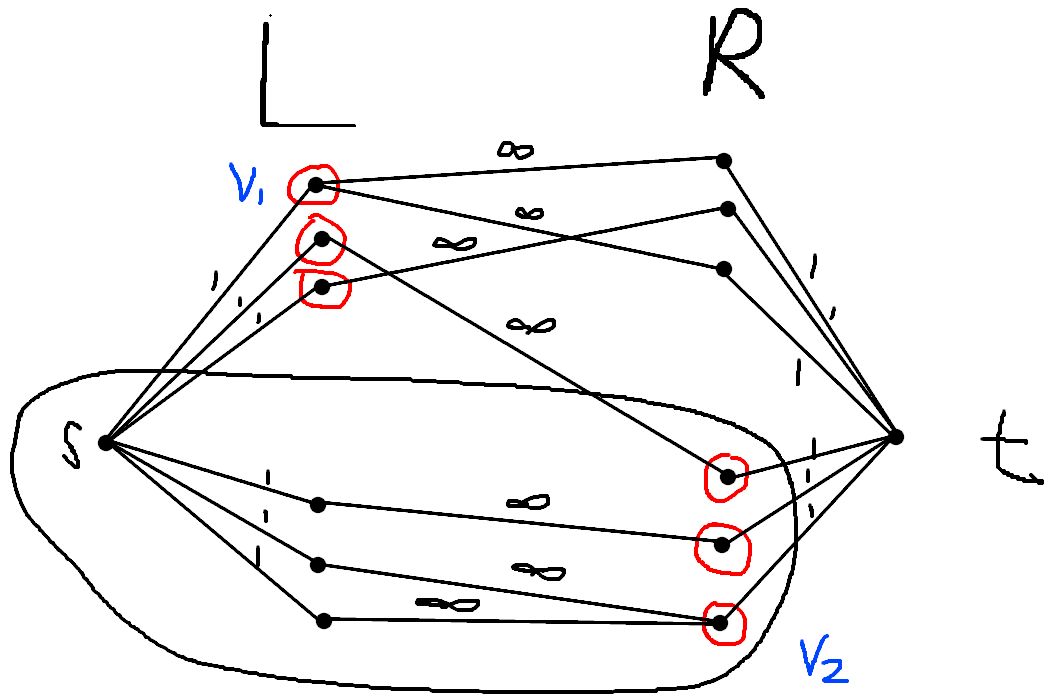
\includegraphics[width=12cm,valign=m]{cscc73-a6-q2-diagram.png}\\
		\footnotesize{Figure 1: a minimum vertex cover (circled in red) with a minimum cut (circled in black)}
	\end{center}~

	This is the minimum cut because the only way to disconnect the flow network is to disconnect $s$ from $L$,
	$L$ from $R$, or $R$ from $t$. We have shown above that $L$ and $R$ are disconnected. Therefore we must include
	all edges from $S$ to $V_1$ and from $V_2$ to $t$ in this cut as well. Otherwise, a path could be made from $s$ to $V_1$ to $R-V_2$ to $t$
	or $s$ to $L-V_1$ to $V_2$ to $t$. Therefore this cut includes all the necessary edges to disconnect the graph while not including
	any $\infty$ weight edges. We know it's the minimum cut since each edge has
	weight 1 and the cut has the only necessary edges.
\end{adjustwidth}~

This is a reduction from vertex cover to max flow min cut because we have shown that an algorithm exists
that takes a bipartite graph and turns it into a flow graph, where the vertex cover can give us the min cut
and a false vertex cover will give us a false min cut.
\newpage
%----------------------------------------------------------------------------------
% !                                     3
%----------------------------------------------------------------------------------
\hyperlink{toc}{\hypertarget{3}{\LARGE \underline{\textbf{Question 3.}}}}\\\\
\begin{algorithm}
  \caption*{\textbf{Algorithm}\\Classify\_Vertices \big(\texttt{G = \{V, E\}}: a flow network, \texttt{s}: start vertex, \texttt{t}: end vertex, \texttt{c}: capacities\big)}\label{alg:cap}
	\begin{algorithmic}[1]
    \State let $(f,\ G_r)$ = Ford-Fulkerson $(G,\ s,\ t,\ c)$
    \State let $(f^\prime,\ {G_r}^\prime)$ = Ford-Fulkerson $(\bar{G},\ t,\ s,\ c)$
    \State
    \State let $u$ be all vertices reachable by $s$ in $G_r$
    \State let $d$ be all vertices reachable by $t$ in ${G_r}^\prime$
    \State let $c$ be $E - u - d$
    \State
    \State return $(u,\ d,\ c)$
	\end{algorithmic}
\end{algorithm}

Proof of complexity:
\begin{adjustwidth}{10mm}{}
	We run Ford-Fulkerson twice, and do 2 BFS's from the 2 start nodes in each residual graph.
	So in total, we have 2$O(m^2 \log c) + 2O(m) \in O(m^2 \log c)$. Therefore, we are still in a
	constant factor of the complexity of Ford-Fulkerson.\\
\end{adjustwidth}

Proof of correctness:
\begin{adjustwidth}{10mm}{}
	\textbf{Lemma 1}: All vertices which are upstream must be reachable from the source of a flow residual
	graph $G_r$ returned by Ford-Fulkerson\\

	Proof of \textbf{Lemma 1} by contradiction
	\begin{adjustwidth}{10mm}{}
		Suppose to the contrary. Then there exist a vertex $u$ that is not reachable from the source $s$ but
		is on the source side of a min cut. Therefore in any min cut, we can find a path in the residual graph
		from an arbitrary vertex $v$ reachable from $s$, to $u$, to $t$ to push flow to create the min cut where $u$ is
		reachable from the source. However, this path connects $s$ to $t$ in the original min cut in the residual graph,
		which is a contradiction. Therefore our assumption is wrong and $u$ must always be reachable from the source in
		any min cut.\\
	\end{adjustwidth}

	By \textbf{Lemma 1}, we can run Ford-Fulkerson and run BFS from $s$ on $G_r$ to get the upstream vertices. \\
	Also by \textbf{Lemma 1}, we can do the same thing with the edges reversed and switching $t$ and $s$
	to get the downstream vertices.\\

	Since we have the upstream and downstream vertices, we can simply
	subtract $u$ and $d$ from $V$ to get all the central vertices. We know that they are central because
	by the definition of a cut, there are vertices reachable by the source, and everything else. Therefore every vertex
	must be in one of the 2 partitions. And since the upstream ones are always on one partition, and the downstream are always
	in the other, the remaining must lie in one of the partitions in some of the cuts, and in the other one in the other cuts.
\end{adjustwidth}
\end{document}
